\documentclass[a4paper,12pt]{article}
\usepackage[utf8]{inputenc}
\usepackage[english]{babel}
\usepackage{graphicx}
\usepackage{listings}
%\usepackage{algpseudocode}
\usepackage[hyphens]{url}
\usepackage[hidelinks]{hyperref}
\usepackage[nottoc,numbib]{tocbibind}
\usepackage{mathtools}
\usepackage{dirtree}
\usepackage{verbatim}
%\usepackage[algoruled,lined,linesnumbered,algochapter]{algorithm2e}
\usepackage[algoruled,lined,linesnumbered]{algorithm2e}
\usepackage[margin=3cm]{geometry}
%\usepackage{algorithm2e}
%\pdfminorversion=7 % fixer en pdf warning
\newcommand{\HRule}{\rule{\linewidth}{0.5mm}}

\newcommand*{\gap}{\text{\textendash}}

\begin{comment}
%% FROM : 
% Alter some LaTeX defaults for better treatment of figures:
    % See p.105 of "TeX Unbound" for suggested values.
    % See pp. 199-200 of Lamport's "LaTeX" book for details.
    %   General parameters, for ALL pages:
    \renewcommand{\topfraction}{0.9}	% max fraction of floats at top
    \renewcommand{\bottomfraction}{0.8}	% max fraction of floats at bottom
    %   Parameters for TEXT pages (not float pages):
    \setcounter{topnumber}{2}
    \setcounter{bottomnumber}{2}
    \setcounter{totalnumber}{4}     % 2 may work better
    \setcounter{dbltopnumber}{2}    % for 2-column pages
    \renewcommand{\dbltopfraction}{0.9}	% fit big float above 2-col. text
    \renewcommand{\textfraction}{0.07}	% allow minimal text w. figs
    %   Parameters for FLOAT pages (not text pages):
    \renewcommand{\floatpagefraction}{0.7}	% require fuller float pages
	% N.B.: floatpagefraction MUST be less than topfraction !!
    \renewcommand{\dblfloatpagefraction}{0.7}	% require fuller float pages
\end{comment}
	% remember to use [htp] or [htpb] for placement
%% END FROM


%----------------------------------------------------------------------------------------
%	TITLE SECTION
%----------------------------------------------------------------------------------------

\newcommand{\horrule}[1]{\rule{\linewidth}{#1}} % Create horizontal rule command with 1 argument of height

\title{	
\normalfont \normalsize 
\textsc{University of Southern Denmark}\\ {DM834 - Bioinformatics I}\\ %[25pt] % Your university, school and/or department name(s)
\horrule{0.5pt} \\[0.4cm] % Thin top horizontal rule
\LARGE {\textbf{Breath Mining}} \\ % The assignment title
\large Intermediate report \\ % The assignment title
\horrule{2pt} \\[0.5cm] % Thick bottom horizontal rule
}

%\author{Anna Bomersbach\\} % Your name
%\begin{flushleft} \large
%\emph{Author:}\\
\author{
\begin{tabular}{rl}
Anna &\textsc{Bomersbach}\\
Felix &\textsc{Drud}\\
Daniel &\textsc{Merino}\\
Mark &\textsc{Reckendorff}\\
Mike &\textsc{Rostermund} 
\end{tabular}
}
%\end{flushleft}
\date{\normalsize\today} % Today's date or a custom date
\begin{document}

\maketitle % Print the title

\begin{comment}

\begin{document}
\begin{titlepage}
\begin{center}
% Upper part of the page
\includegraphics[width=0.55\textwidth]{logo.pdf}\\[1cm]
\textsc{\LARGE University of Southern Denmark}\\[1.5cm]
\textsc{\Large Bioinformatics I}\\[0.5cm]
% Title
\HRule \\[0.4cm]
{ \huge \bfseries Breath Mining}\\[0.4cm]
\HRule \\[1.5cm]
% Author and supervisor
\begin{minipage}{0.4\textwidth}
\begin{flushleft} \large
\emph{Author:}\\
Anna \textsc{Bomersbach}\\
Felix \textsc{Drud}\\
Daniel \textsc{Merino}\\
Mark \textsc{Reckendorff}\\
Mike \textsc{Rostermund}
\end{flushleft}
\end{minipage}
\begin{minipage}{0.4\textwidth}
\begin{flushright} \large
\emph{Supervisor:} \\
Associate Professor\\Jan \textsc{Baumbach}\\
\vspace{4mm}
\emph{Teaching Assistants:}\\
Markus \textsc{List}\\
Eudes \textsc{Barbosa}
\end{flushright}
\end{minipage}
\vfill
% Bottom of the page
{\large \today}
\end{center}
\end{titlepage}

\newpage


\end{comment}

% !TEX root = ./main.tex
\section{Status}
Until now we have been using a combination of Bash, Python and R. Preprocessing is done in Python, while the plots have been done in R. To run the preprocessing and then perform the plots, a few Bash scripts have been created. Tests have been performed using the labelled raw data. An example of a density plot has been included, see figure~\ref{fig:density}.

When finding the peak ID's, we used the euclidean distance for the distance measure. The first input file would become the baseline for the peaks. When reading some peak, we search in the baseline to find the peak that is closest to the new peak. If the closest peak is below the threshold it will get the same ID, if not then it would get a new peak ID. We plan to implement a method in the next few weeks that performs k-Means clustering on the data to find the peak ID's.

The indicator matrix is created by going through the output of finding the peak ID's and formatting it as an indicator matrix with samples on one dimension and peaks on the other dimension. The value at a given place of the indicator matrix would indicate whether the sample contains the peak or not.

At this point we are looking at using the package \texttt{randomForest} in R with the indicator matrix. After this, we will be looking at the package \texttt{cvTools} in R for cross-validation.
\newpage
\begin{figure}[h]
\centering
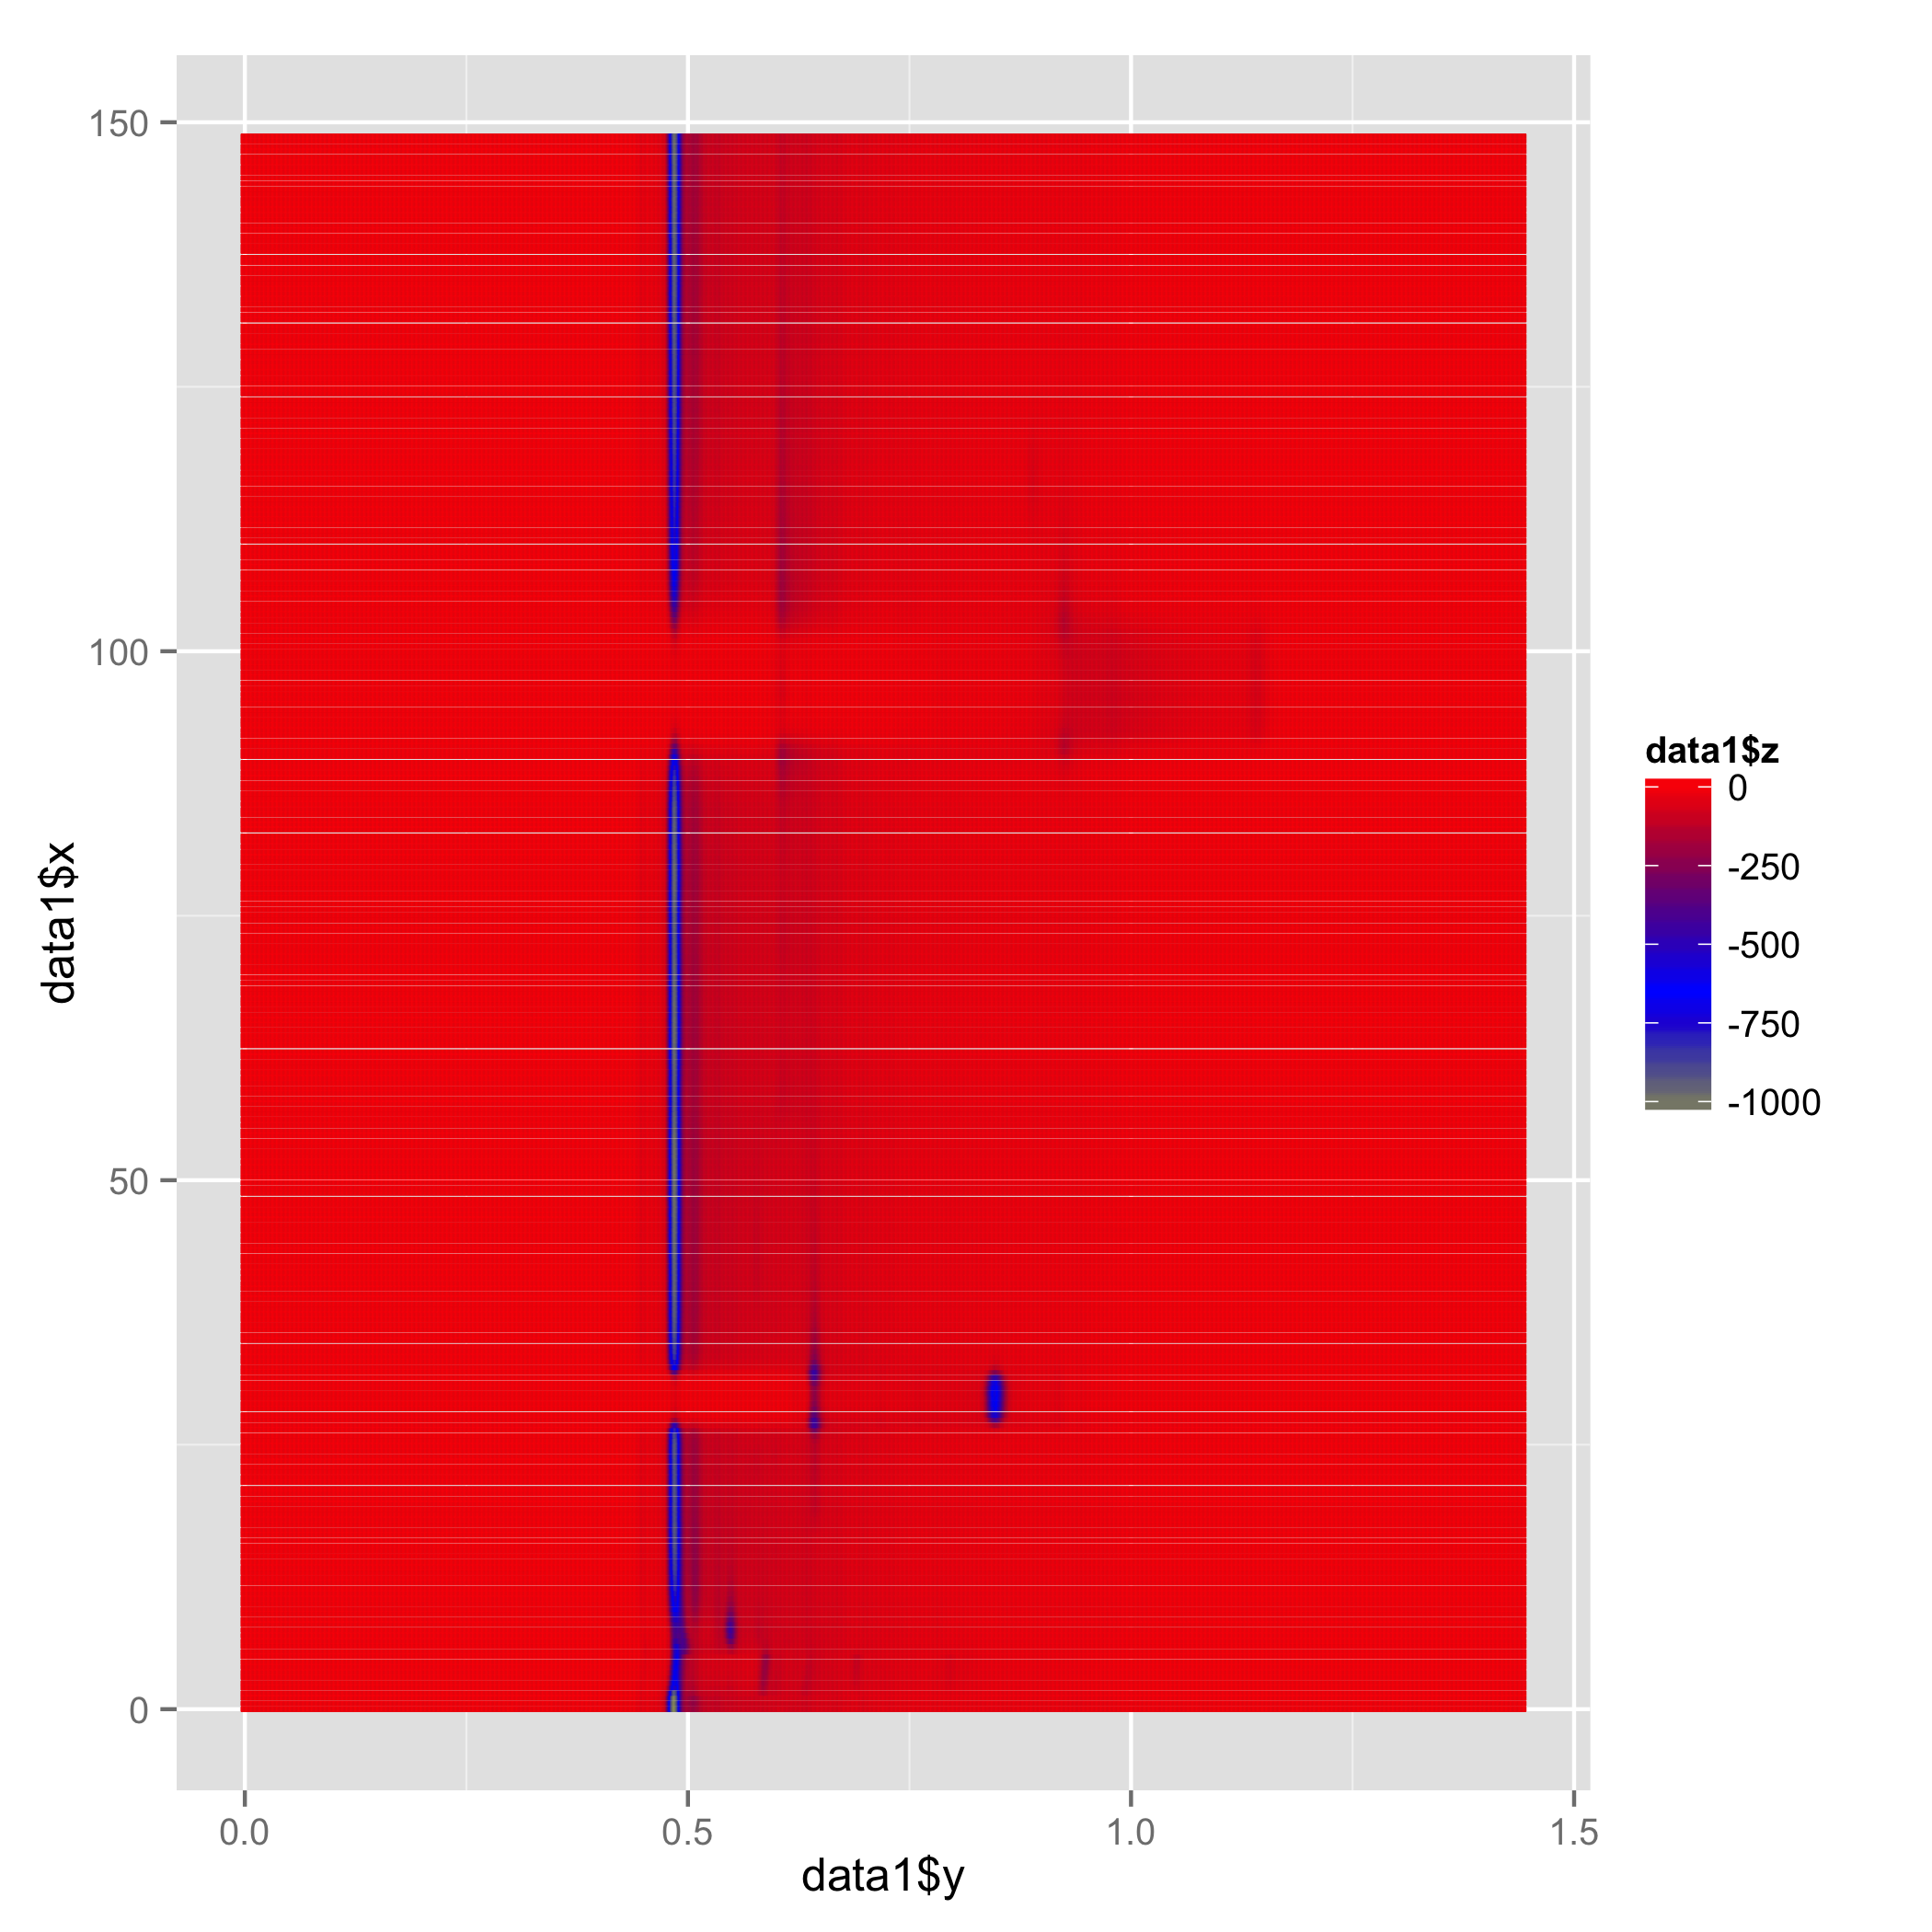
\includegraphics[width=1.00\textwidth]{../../plots/density/BD18_1411061750_ims.png}
\caption{Density plot for sample \texttt{BD18\_1411061750}.}
\label{fig:density}
\end{figure}

\begin{figure}[h]
\centering
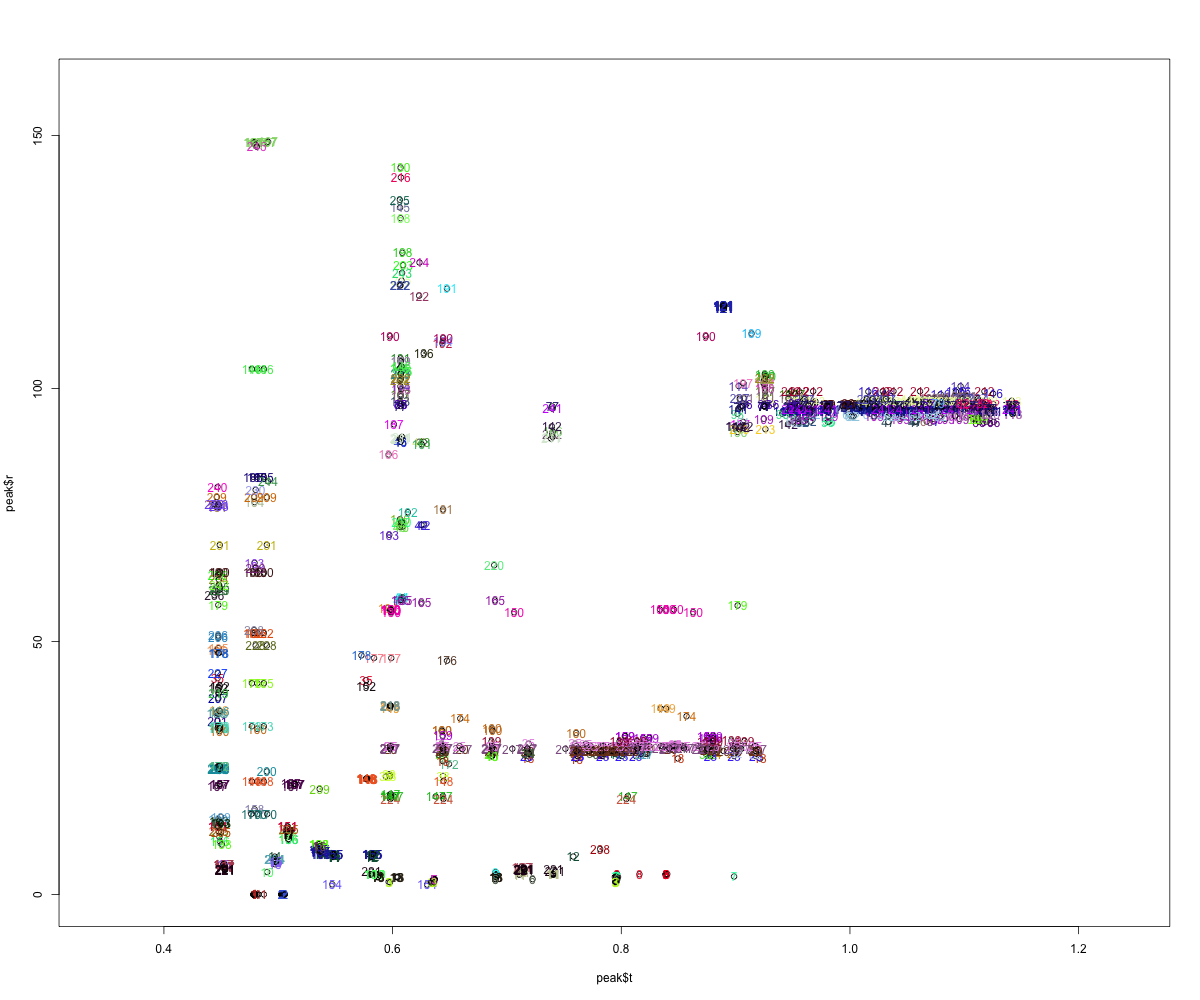
\includegraphics[width=1.00\textwidth]{../../plots/peak/peakoutput.png}
\caption{Peak alignment plot.}
\label{fig:peak_align}
\end{figure}

\begin{figure}[h]
\centering
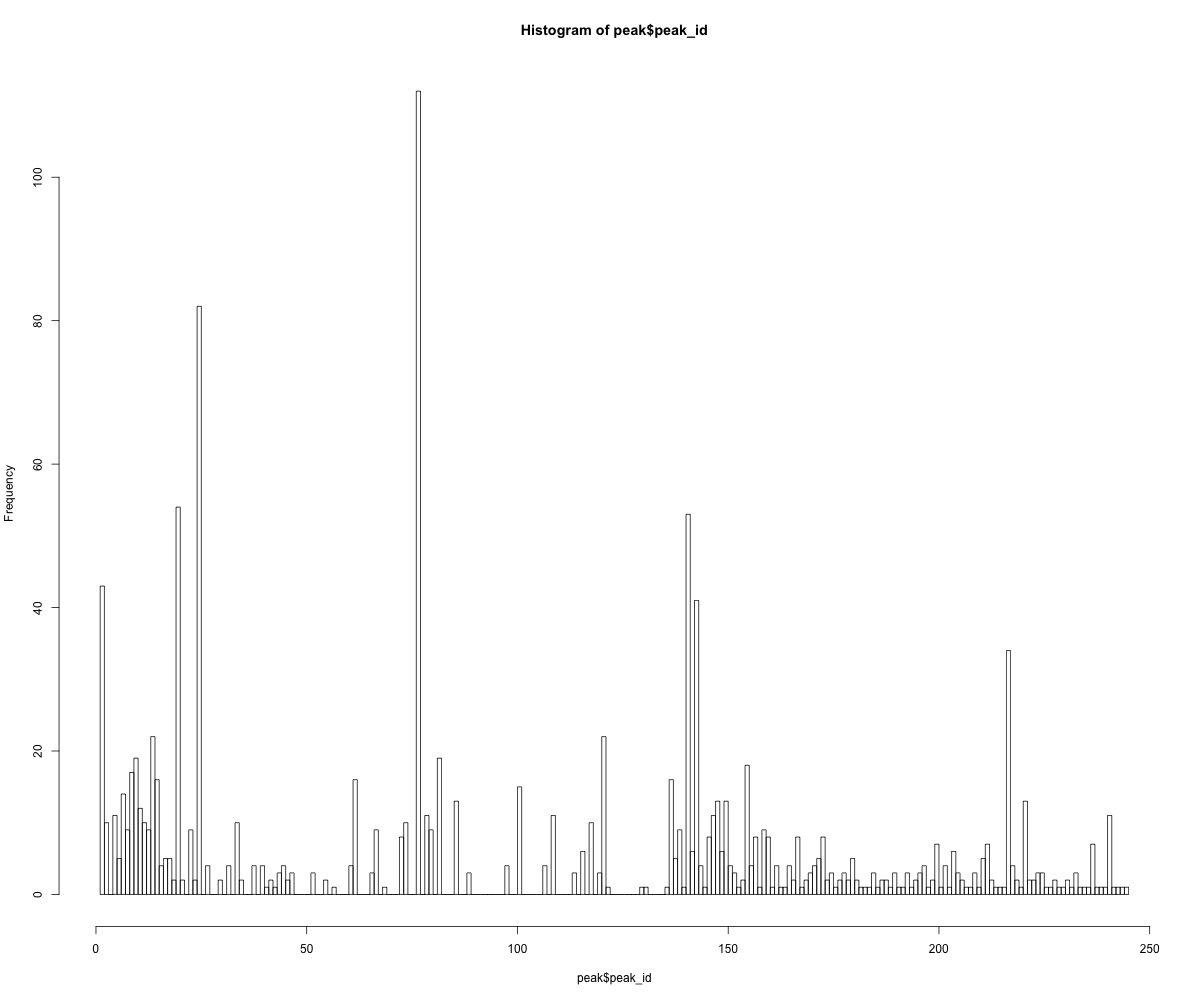
\includegraphics[width=1.00\textwidth]{../../plots/peak/peakoutput_histogram.png}
\caption{Histogram of peak ID's.}
\label{fig:peak_hist}
\end{figure}



\end{document}
